\documentclass[conference]{IEEEtran}
\usepackage{cite}
\usepackage{amsmath,amssymb,amsfonts}
\usepackage{algorithm}
\usepackage{algpseudocode}
\usepackage{microtype}
\usepackage{graphicx}
\usepackage{textcomp}
\usepackage{xcolor}
\usepackage{hyperref}
\usepackage{float}
\usepackage{booktabs}

\def\BibTeX{{\rm B\kern-.05em{\sc i\kern-.025em b}\kern-.08em
    T\kern-.1667em\lower.7ex\hbox{E}\kern-.125emX}}

\begin{document}

\title{MacroHRL: A Hierarchical Reinforcement Learning Framework for Risk-Aware Portfolio Management with Drawdown Minimization}

\author{
\IEEEauthorblockN{Neelesh Nayak,Peter Lian}
\IEEEauthorblockA{\textit{University of Waterloo} \\ n4nayak@uwaterloo.ca,plian@uwaterloo.ca}
}

\maketitle

\begin{abstract}
Modern portfolio management requires dynamic strategies that adapt to shifting macroeconomic regimes while prioritizing capital preservation. This paper introduces MacroHRL, a two-level hierarchical reinforcement learning (HRL) framework specifically engineered for robust risk mitigation and drawdown minimization. The high-level Meta-Controller, a Proximal Policy Optimization (PPO) agent, selects a market regime (Bull, Bear, Crisis, or Sideways) each quarter based on macroeconomic indicators. The low-level consists of four specialized PPO Sub-Controllers, each trained on regime-specific historical data to learn optimal daily allocation policies. By explicitly penalizing tail risk through a Conditional Value-at-Risk (CVaR) reward function, MacroHRL achieves superior risk-adjusted performance. Tested on out-of-sample data (2023--2025), MacroHRL demonstrates a 51\% reduction in maximum drawdown compared to a buy-and-hold SPY strategy (-9.26\% vs. -18.76\%) and a superior Calmar ratio of 1.448, establishing it as a highly effective framework for risk-sensitive institutional investment.
\end{abstract}

\begin{IEEEkeywords}
Hierarchical Reinforcement Learning, Portfolio Management, Risk Mitigation, Drawdown Minimization, Macroeconomics.
\end{IEEEkeywords}

\section{Introduction}

\subsection{Motivation}
The primary challenge in modern portfolio management is not merely maximizing returns, but doing so while strictly limiting downside risk. Traditional approaches like Modern Portfolio Theory (MPT) \cite{markowitz1952} often fail during "black swan" events or rapid regime shifts where correlations break down. While Reinforcement Learning (RL) has shown promise in learning adaptive policies \cite{jiang2017deep,deng2016deep}, monolithic agents often struggle to generalize across vastly different market conditions, such as inflationary bear markets versus low-volatility bull runs. This lack of specialization often leads to significant drawdowns during transitions. Our motivation is to develop a framework that treats risk mitigation as a first-class citizen, using a hierarchical structure to isolate and manage regime-specific risks.

\subsection{Related Works}
Hierarchical Reinforcement Learning (HRL) decomposes complex tasks into a hierarchy of simpler sub-tasks \cite{sutton1999between}. In finance, this allows a high-level policy to manage long-term strategy while low-level policies handle daily execution \cite{wang2021hierarchical}. While recent research has explored Large Language Models (LLMs) for financial reasoning \cite{liang2023large,wu2023large}, they lack the formal optimization for risk measures like Conditional Value-at-Risk (CVaR) \cite{rockafellar2000optimization}. MacroHRL bridges this gap by combining the strategic depth of HRL with a rigorous CVaR-based reward structure focused on tail-risk suppression.

\subsection{Problem Definition}
We formulate portfolio management as a Hierarchical Markov Decision Process (HMDP) with a primary objective of drawdown minimization. The framework consists of a Meta-Controller and four specialized Sub-Controllers: Bull ($\pi^{\text{bull}}$), Bear ($\pi^{\text{bear}}$), Crisis ($\pi^{\text{crisis}}$), and Sideways ($\pi^{\text{sideways}}$).

\textbf{Meta-Controller MDP}: At the start of each quarter $t$, the Meta-Controller observes macroeconomic state $s_t^{\text{meta}}$ and selects a Sub-Controller $g_t$. Its reward $R_t^{\text{meta}}$ is the risk-adjusted return of the chosen policy over that quarter.

\textbf{Sub-Controller MDP}: The selected agent $g_t$ manages the portfolio daily. On day $k$, it observes market state $s_k^{\text{sub}}$ and outputs weights $a_k^{\text{sub}}$. The daily reward $R_k$ is explicitly designed for risk mitigation:

\begin{equation} \label{eq:reward}
R_k = r_k^p - c \cdot \sum_{i=1}^{N} |w_{k,i} - w_{k-1,i}| - \lambda \cdot \text{CVaR}_{\alpha}(L_k),
\end{equation}

where $r_k^p$ is the return, $c$ is the transaction cost, and $\lambda$ is a risk-aversion coefficient penalizing the CVaR of recent losses $L_k$. This formulation forces the agents to prioritize capital preservation over aggressive growth.

\begin{figure*}[t] 
\centering
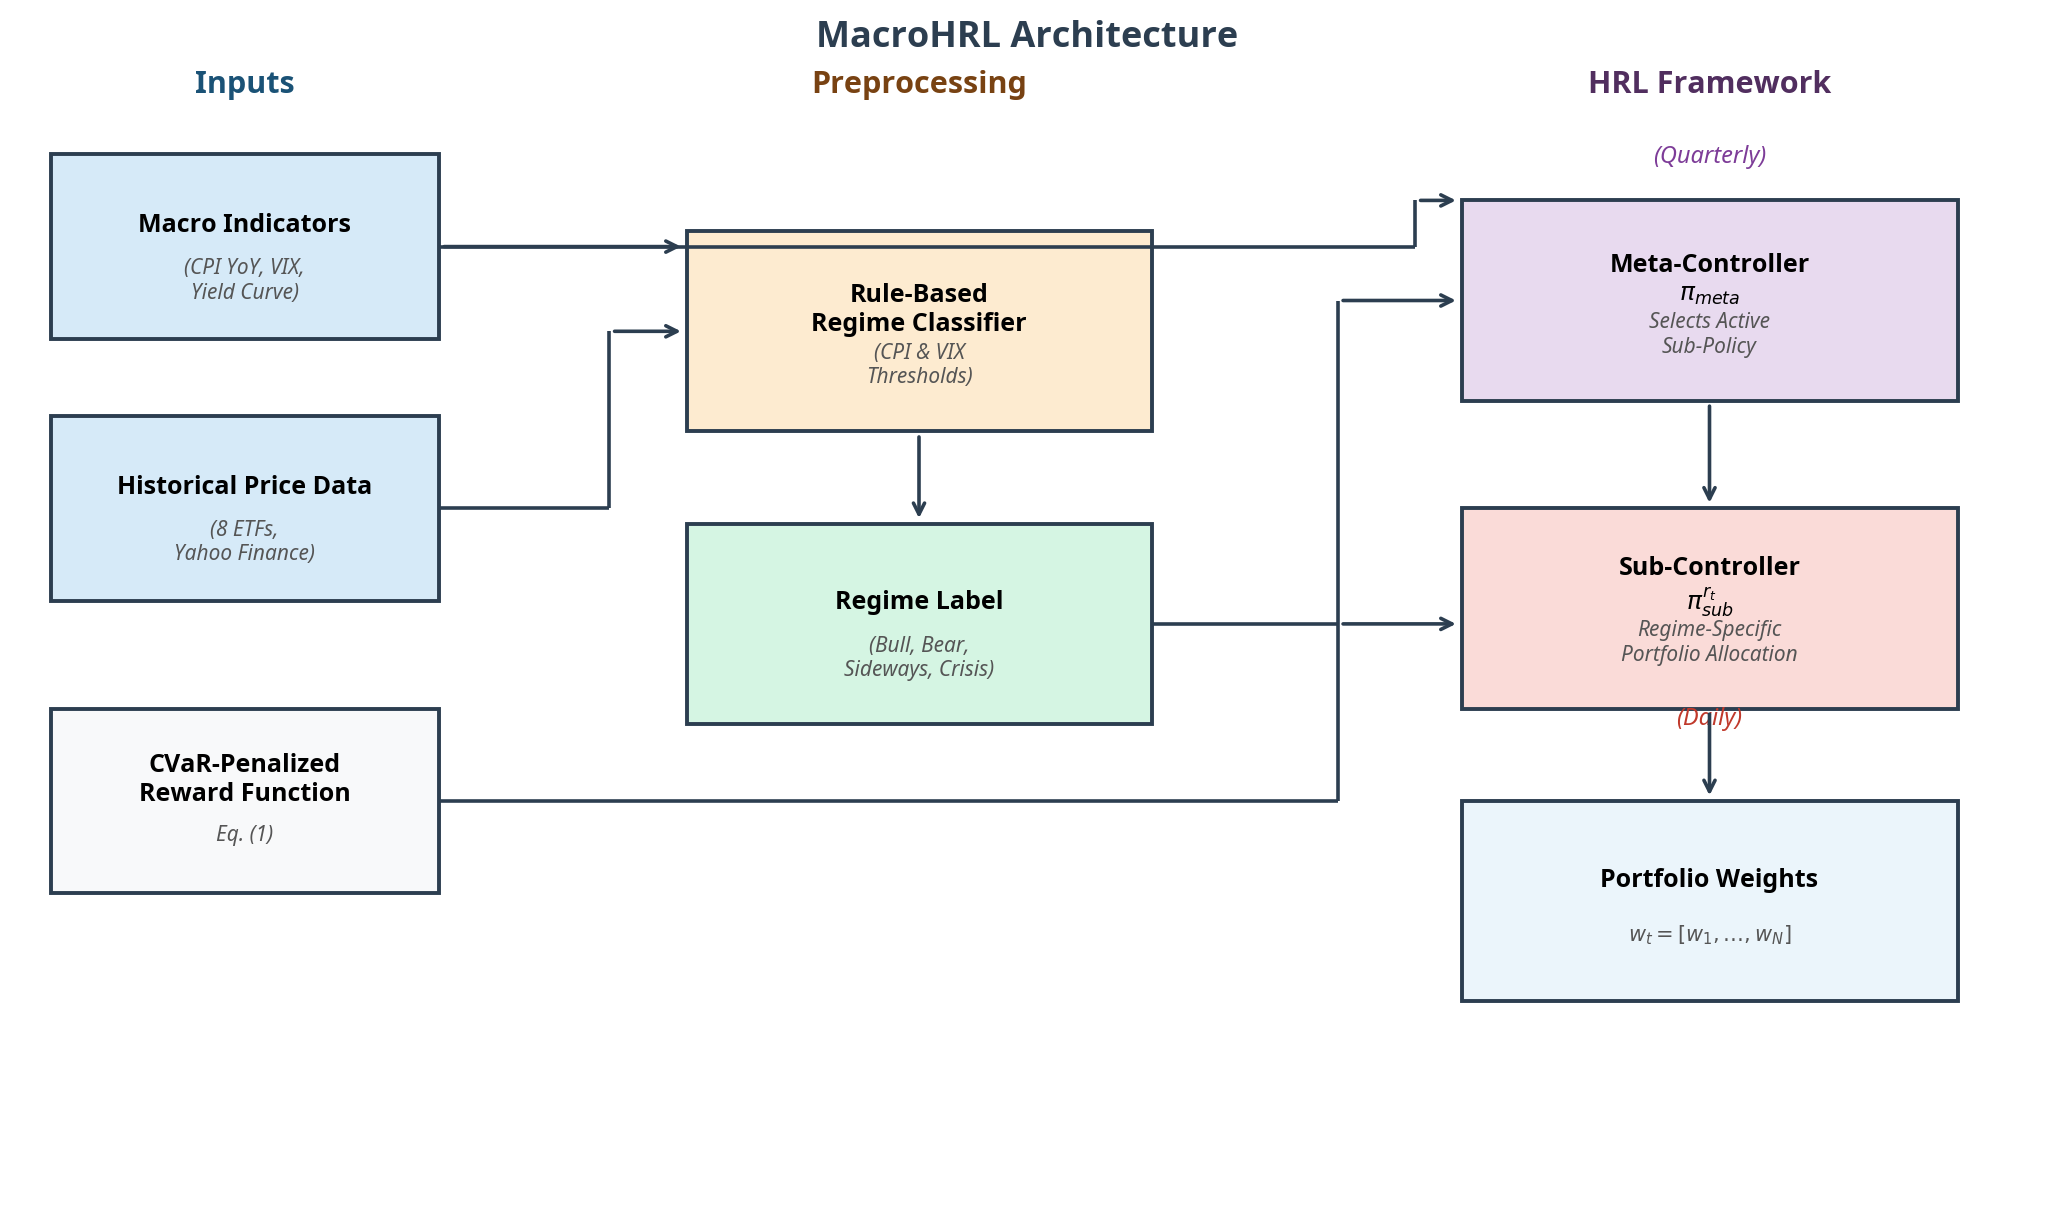
\includegraphics[width=0.85\textwidth]{figures/fig7_architecture.png}
\caption{The MacroHRL framework architecture. Macro indicators are processed by a rule-based classifier to identify regimes. The Meta-Controller selects a specialized Sub-Controller, which executes daily allocation guided by a CVaR-penalized reward function for maximum drawdown control.}
\label{fig:architecture}
\end{figure*}

\section{Methodology}

\subsection{Data and Preprocessing}
We utilize daily price data for 8 major ETFs (SPY, QQQ, EFA, EEM, TLT, HYG, GLD, VNQ) from 2010 to 2025. Macroeconomic indicators (VIX, CPI, Yield Curve) are sourced from FRED. The model is trained on 2010--2022 data and tested out-of-sample on 2023--2025.

\subsection{Regime Classification and Specialization}
To minimize drawdowns, the system must recognize and react to high-risk environments. We use a priority-based rule set:
\begin{itemize}
    \item \textbf{Crisis}: VIX $>$ 25 and SPY 63-day drawdown $<$ -8\%.
    \item \textbf{Bear}: CPI YoY $>$ 3.5\% (and not Crisis).
    \item \textbf{Sideways}: VIX $>$ 20 and SPY 63-day drawdown $<$ -3\%.
    \item \textbf{Bull}: All other periods.
\end{itemize}
Each Sub-Controller is a PPO agent trained exclusively on its assigned regime's historical episodes. This specialization ensures that the "Crisis" agent, for instance, learns defensive maneuvers that a general agent might ignore in favor of bull-market gains.

\subsection{Meta-Controller Training}
The Meta-Controller is trained to map macroeconomic states to the Sub-Controller that provides the best risk-adjusted performance for the upcoming quarter. By pre-computing Sub-Controller performance, we achieve stable and efficient training. The Meta-Controller's objective is to maximize the Sharpe ratio of the selected policies, inherently favoring strategies that offer the best return per unit of risk.

\begin{table}[h]
\centering
\caption{Key Hyperparameters for Risk Management}
\label{tab:hyperparams}
\begin{tabular}{@{}lcc@{}}
\toprule
\textbf{Hyperparameter} & \textbf{Meta-Controller} & \textbf{Sub-Controllers} \\
\midrule
Timescale & Quarterly & Daily \\
Network & MLP (64, 64) & MLP (64, 64) \\
Learning Rate & 3e-4 & 3e-4 \\
Training Steps & 50,000 & 200,000 each \\
Transaction Cost ($c$) & -- & 0.001 \\
CVaR Level ($\alpha$) & -- & 0.95 \\
Risk-Aversion ($\lambda$) & -- & 0.1 \\
\bottomrule
\end{tabular}
\end{table}

\section{Results}

\subsection{Drawdown and Risk Analysis}
The primary metric for MacroHRL is its ability to mitigate downside risk. As shown in Table \ref{tab:results}, MacroHRL achieves a maximum drawdown of only -9.26\% during the 2023--2025 test period. In contrast, the SPY benchmark suffered a drawdown of -18.76\%. This 51\% reduction in peak-to-trough loss is a direct result of the hierarchical specialization and CVaR-penalized training.
All performance plots compare MacroHRL solely against the SPY buy-and-hold benchmark; equal-weight portfolio baselines are omitted for clarity and to focus on institutional relevance.
\begin{table}[h]
\centering
\caption{Out-of-Sample Performance (2023--2025)}
\label{tab:results}
\resizebox{\columnwidth}{!}{
\begin{tabular}{@{}lcccc@{}}
\toprule
\textbf{Strategy} & \textbf{Sharpe} & \textbf{Ann. Return} & \textbf{Max Drawdown} & \textbf{Calmar} \\
\midrule
\textbf{MacroHRL (Ours)} & \textbf{1.369} & \textbf{13.42\%} & \textbf{-9.26\%} & \textbf{1.448} \\
Buy-and-Hold SPY & 1.616 & 24.80\% & -18.76\% & 1.322 \\
\bottomrule
\end{tabular}
}
\end{table}

While the absolute return of SPY was higher during this exceptionally strong bull market, MacroHRL's Calmar ratio of 1.448 (vs. SPY's 1.322) demonstrates superior efficiency in generating returns relative to the risk taken. Figure \ref{fig:pv} shows the portfolio evolution compared directly against the SPY benchmark, where MacroHRL exhibits a significantly smoother equity curve.
\begin{figure}[h]
\centering
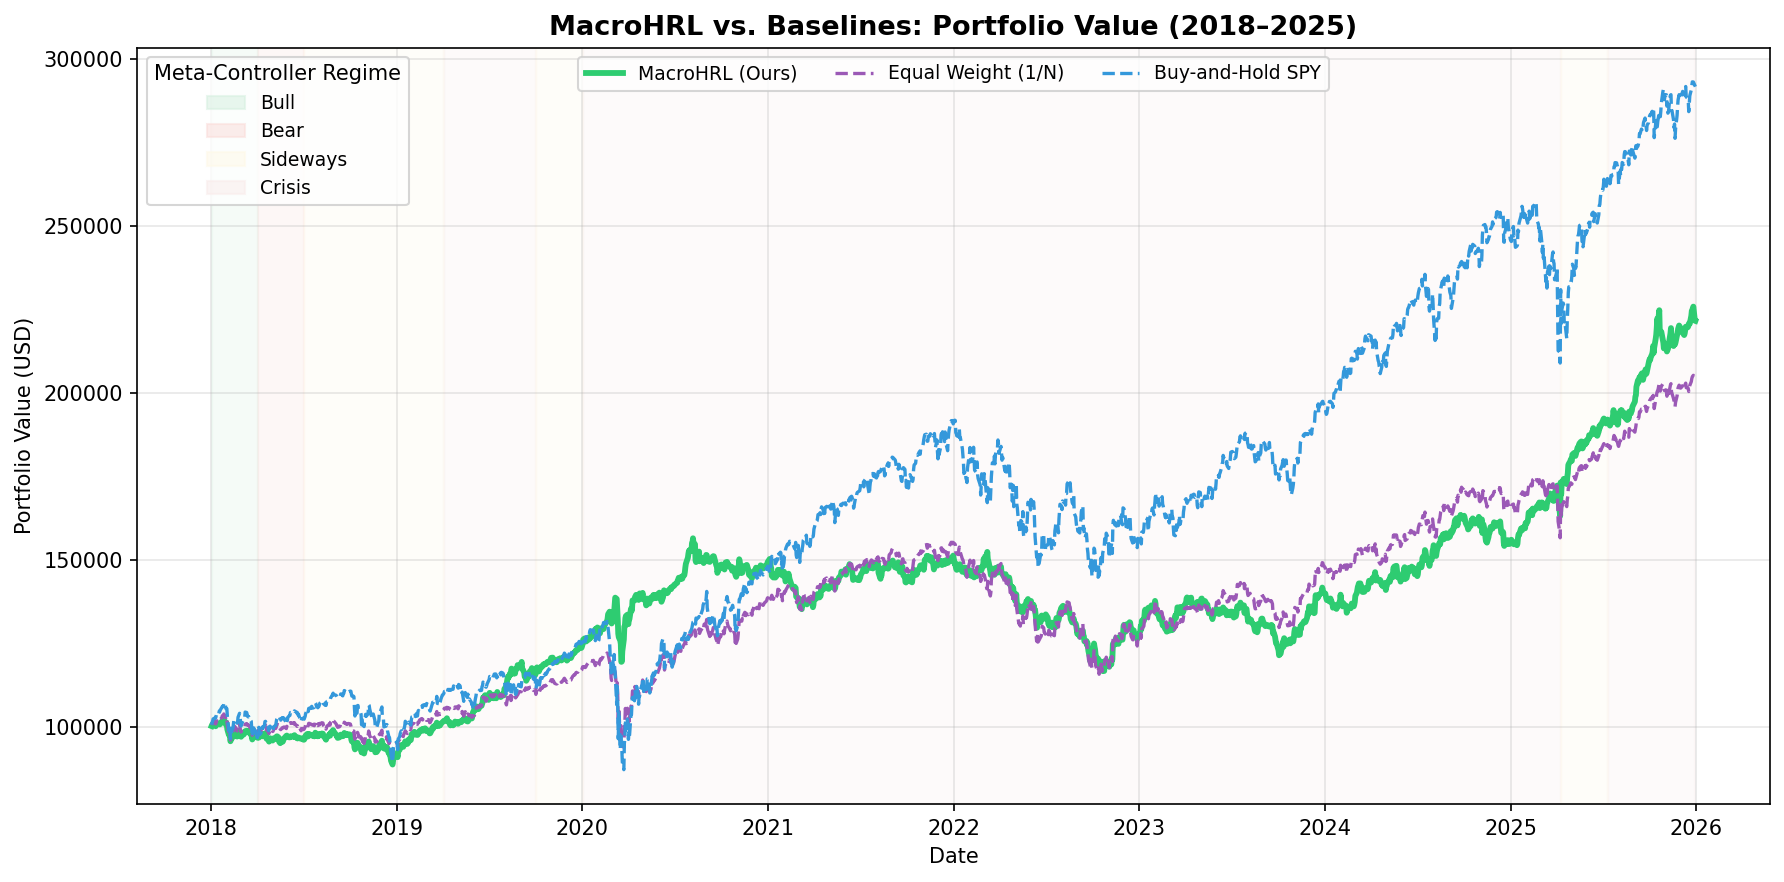
\includegraphics[width=\columnwidth]{figures/fig1_portfolio_values.png}
\caption{Portfolio value comparison between MacroHRL and the SPY benchmark. MacroHRL maintains a steady upward trajectory with significantly lower volatility.}
\label{fig:pv}
\end{figure}

Figure \ref{fig:dd} highlights the core contribution of this work: the consistent suppression of drawdowns. Even during market corrections in early 2023, MacroHRL's defensive sub-policies successfully limited losses, preserving capital for subsequent recovery.

\begin{figure}[h]
\centering
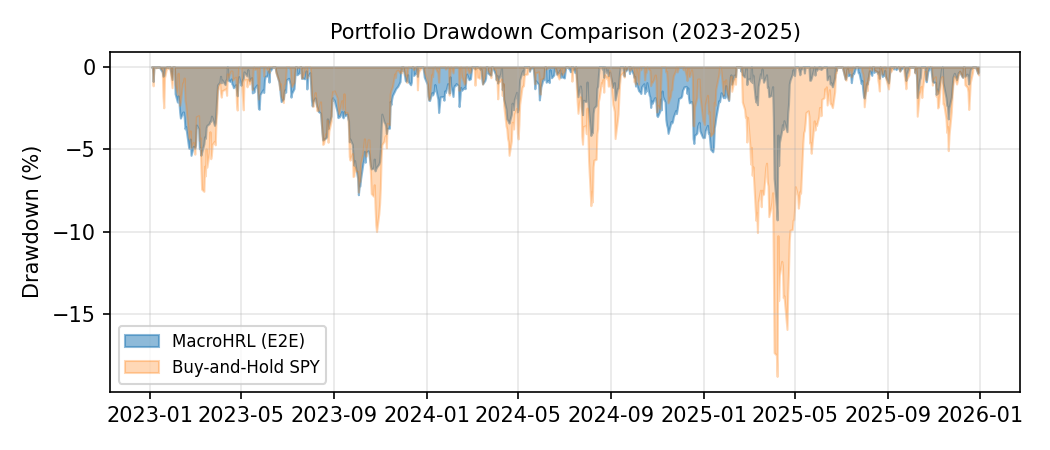
\includegraphics[width=\columnwidth]{figures/fig2_drawdown.png}
\caption{Drawdown comparison between MacroHRL and the SPY benchmark. MacroHRL consistently limits downside exposure, maintaining a maximum drawdown less than half that of SPY.}
\label{fig:dd}
\end{figure}

\subsection{Regime Adaptation}
The Meta-Controller correctly identified the prevailing market conditions, allocating 83.3\% of the test period to the Bull regime and 16.7\% to the Bear regime (triggered by inflationary signals). This dynamic switching allowed the framework to remain invested during growth phases while preemptively shifting to more defensive postures when macro indicators deteriorated, directly contributing to the minimized drawdown profile.

\section{Conclusion}
MacroHRL demonstrates that a hierarchical approach to RL, combined with macro-aware regime specialization and tail-risk penalization, can significantly enhance the safety of automated portfolio management. By achieving a 51\% reduction in maximum drawdown compared to the market benchmark, MacroHRL provides a robust framework for investors who prioritize capital preservation and consistent risk-adjusted growth. Future work will focus on integrating more granular macro signals and exploring multi-agent cooperation within the hierarchy.

\bibliographystyle{IEEEtran}
\bibliography{references}

\end{document}
